\chapter{Problem Definition}
    \label{chap:defproblem}
    This Chapter is dedicated to fundamental concepts and definitions in the Reinforcement Learning field. At first, Section \ref{defproblem:mdp} is concerned with the presentation of the Markov Decision Process framework, along with all the notions that are necessary as basic building blocks for this research. In the second part, Section \ref{defproblem:delays} offers a more detailed description of the concept of Delays in Reinforcement Learning and its interaction with the MDP framework is explicitly described, in order to provide a solid base of knowledge for Chapter \ref{chp:sota} and the rest of thesis, since it represents the problem it aims to solve. 
    
    \section{Markov Decision Process Framework}
        \label{defproblem:mdp}
        Markov Decision Process (MDP) is the fundamental framework for modeling the problem of learning through interaction with an environment in order to achieve a defined goal. The entity that represents the decision maker is called Agent, while the entity that represents everything the Agent can interact with is called Environment. Throughout this section, MDPs are defined with all elements and overall functioning, representing ground knowledge for the rest of the research thesis. Notions presented in this section can be referred to in \pcite{rl:mdp}.
        
        \begin{figure}[t]
            \centering
            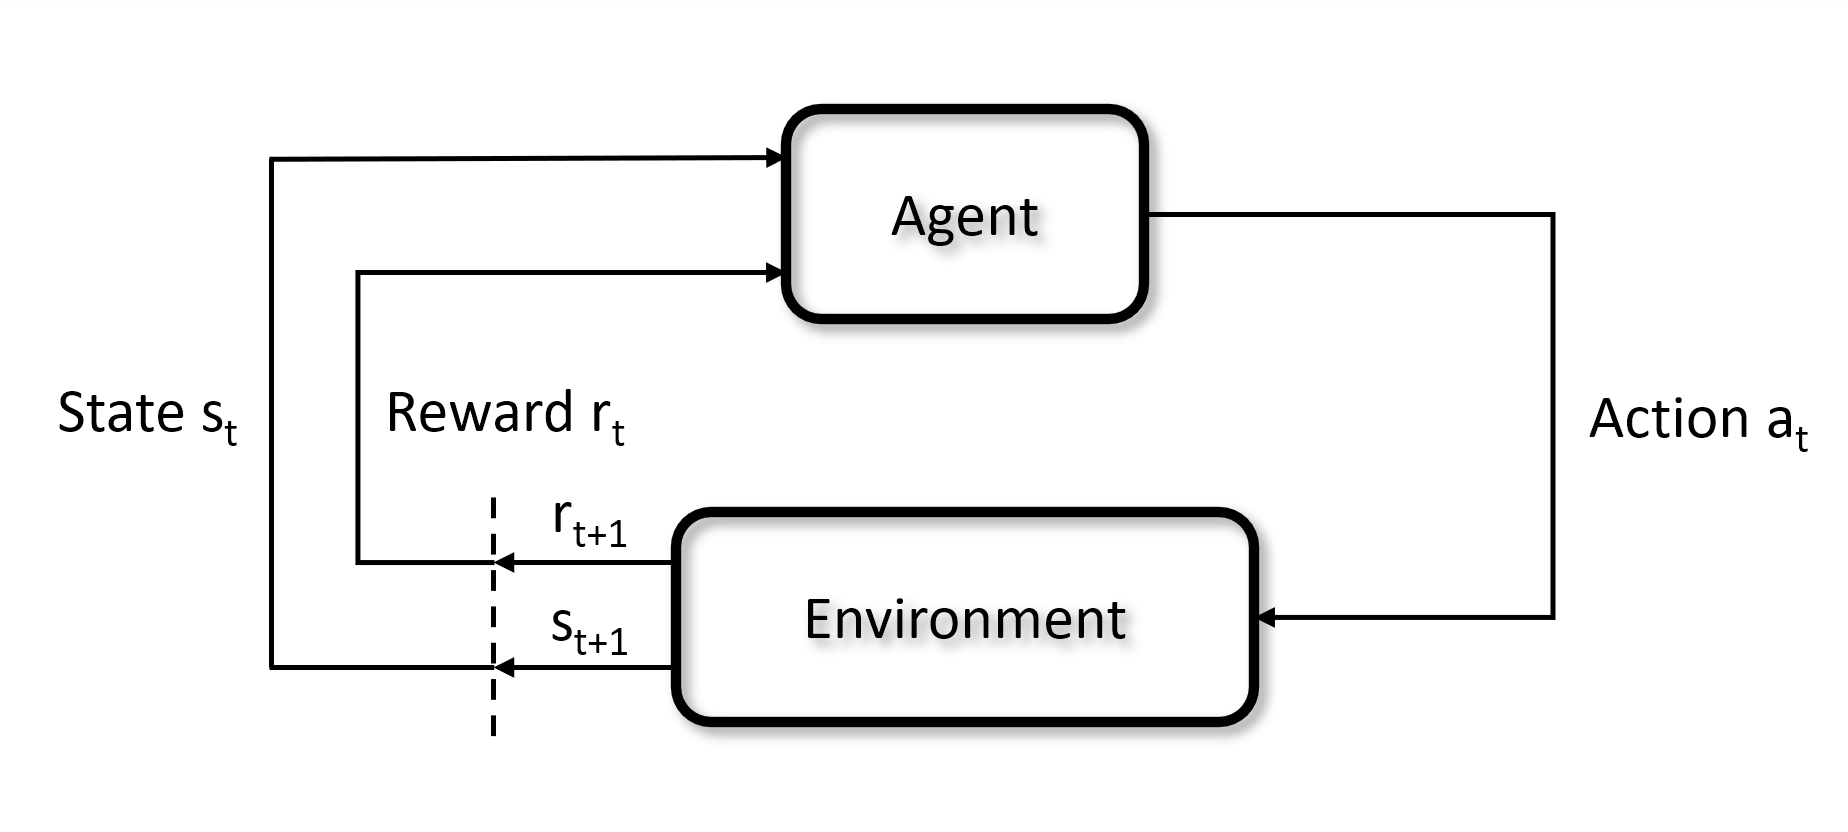
\includegraphics[width=14cm, keepaspectratio]{images/mdp/int_schema.png}
            \caption{A schema of the Agent-Environment Interaction.}
            \label{fig:mdp}
        \end{figure}
        
        \subsection{State, Action and Reward}
            \label{subs:sar}
            The interaction between the Agent and the Environment is articulated in a sequence of discrete time-steps. At each time-step \textit{t}, the Agent receives a representation of the Environment, called State ($s_t\in \mathbf{S}$). Then the Agent selects an Action ($a_t\in \mathbf{A}$)  to be executed in the Environment. As a consequence of the aforementioned Action $a_t$, at time-step \textit{t+1} the Agent receives a Reward ($r_{t+1}\in \mathbf{R}$) and perceives a new State $s_{t+1}$. The cyclic nature of this behavior can be observed in Figure \ref{fig:mdp}. 
            \\\\
            The interaction between the Agent and the Environment along the time-steps produces a trajectory: $s_0, a_0, r_1, s_1, a_1, r_2, s_2, ...$, which can be finite or infinite depending on the Time Horizon of the MDP.
            \\\\
            The set of all states $\mathbf{S}$ is called State Space, the set of all actions $\mathbf{A}$ is called Action Space. States and actions can be either Discrete or Continuous depending on the Environment properties. At last, $\mathbf{R}$ is the Reward Function, which returns a reward for each triple $(s, a, s')$ and thus can be defined as: $\mathbf{R}: \mathbf{S} \times \mathbf{A} \times \mathbf{S} \rightarrow \mathds{R}$.
            
        \subsection{Markov Property and State-Transition Probabilities}
            \label{subs:markov}
            A defining property of the Markov Decision Process is the Markov Property, which states: 
            
            \begin{definition}[Markov Property]
                \label{def:markov}
                A stochastic process $S_{t}$ is said to be Markovian if and only if:
                \[ P \left( S_{t+1} = s' | S_{t} = s, S_{t-1} = s_{t-1}, ..., S_{1} = s_1, S_{0} = s_0 \right) = P \left( S_{t+1} = s' | S_{t} = s \right)\]
                
                where the stochastic process $S_t$ is the trajectory the Agent follows in the environment. Therefore the State $s$ constitute a sufficient statistic for the future sequence of states.
            \end{definition}
            \noindent
            Intuitively, the Markov Property states that each state $s$ must include all necessary information and aspects of the interaction between the Agent and the Environment that occurred before the Agent reached the said state and previous history is not needed in order to plan future actions. \newline
            This property has fundamental consequences since it enables decision-making that relies only on the knowledge of the current state and reward and not on the full trajectory experienced by the Agent. Upon this property, the Dynamics of the MDP can be defined as: 
            
            \begin{definition}[Dynamics of the MDP]
                \label{def:dynamics}
                \[P : \mathbf{S} \times \mathbf{A} \times \mathbf{S} \times \mathbf{R} \rightarrow [0, 1] \]
                \[P(s', r | s, a) \doteq \mathbf{E} \left[S_{t+1}=s', R_{t+1}=r | S_t=s, A_t=a \right]\]
            \end{definition}
            \noindent
            Thus, the probability of the Agent reaching a new state $s_{t+1}$ receiving a reward $r_{t+1}$ only depends on the previous state $s_t$ and the following action $a_t$. The entire trajectory traversed by the Agent so far is not necessary. The dynamics of the MDP define the entire behaviour of the interaction.
            \\\\
            At last, derived from the Dynamics of the system, the State-Transition Probability Function defines the probability of reaching a certain new state $s_{t+1}$ knowing the current state $s_t$ and action $a_t$:
            
            \begin{definition}[State-Transition Probability Function]
                \label{def:transprob}
                \[p : \mathbf{S} \times \mathbf{A} \times \mathbf{S} \rightarrow [0, 1] \]
                \[ p(s' | s, a) \doteq \sum_{r\in \mathbf{R}} P(s', r | s, a) \]
            \end{definition}
            \noindent
            State transitions can be either Deterministic or Stochastic, depending on the values of the State-Transition Probability Function, and thus, ultimately, on the Dynamics of the system. Deterministic State-Transition Probability functions assigns to each triple $(s, a, s')$ either probability 0 or probability 1, denoting a rather simple Environment in which each action provides clear and repeatable results. Stochastic State-Transition Probability functions, instead, assigns continuous probability values to each triple $(s, a, s')$, denoting a more complex environment in which actions' consequences are variable in each state. \newline
            To shorten the notation, an Environment characterized by Deterministic State-Transition Probability function can be simply called Deterministic Environment and, analogously, Stochastic Environments can be defined. \newline
            Intuitively, learning in a Deterministic Environment is much simpler than in a Stochastic Environment, due to the fact that the decisions taken by the Agent will have fixed and repeatable consequences. In Stochastic Environment, instead, selecting the same action $a$ twice in the same state $s$ may lead to different next states $s'$ and, as a consequence, the Agent will need more experience in the Environment in order to correctly assess all possible outcomes.
            
        \subsection{Markov Decision Process}
            Now that all its components have been presented, a formalized definition of a Markov Decision Process can be given:
            
            \begin{definition}[Markov Decision Process (MDP)]
                \label{def:mdp}
                A Markov Decision Process (or MDP) is a 4-tuple:
                \[ \langle \mathbf{S}, \mathbf{A}, p, \mathbf{R} \rangle\]
                where:
                \begin{itemize}
                    \setlength\itemsep{0em}
                    \item $\mathbf{S}$ is the set of states, called State Space;
                    \item $\mathbf{A}$ is the set of actions, called Action Space;
                    \item $p$ is the State-Transition Probability function;
                    \item $\mathbf{R}$ is the Reward function.
                \end{itemize}
            \end{definition}
            
        \subsection{Policy, Value and Action-Value Functions}
            \label{subs:PVQ}
            
            \begin{figure}[t]
                \centering
                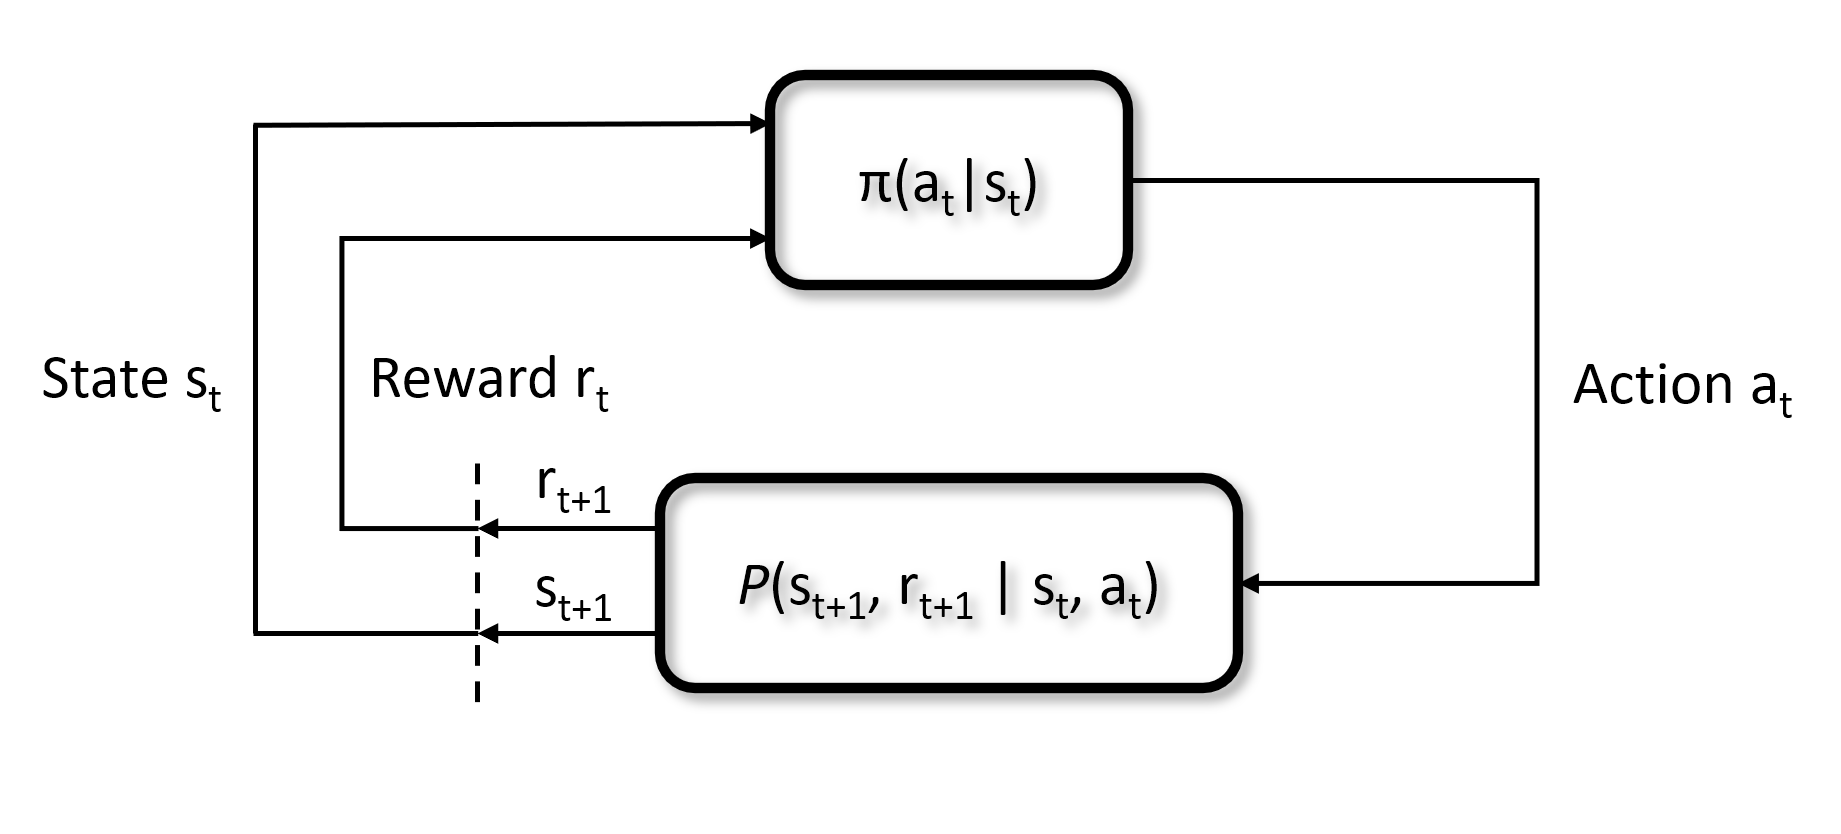
\includegraphics[width=14cm, keepaspectratio]{images/mdp/int_schema_def.png}
                \caption{A schema of the Agent-Environment Interaction denoting the purpose of the Policy Function $\pi$ and Dynamics of the System $P$.}
                \label{fig:int_schema_def}
            \end{figure}
            
            As described so far, the Environment evolution through time is guided by the Dynamics of the MDP, while the Agent is able to choose an action at each step of the trajectory, traversing different states in order to reach its goal, which is defined by the reward function. 
            
            \begin{definition}[Policy]
                \label{def:policy}
                A Policy is a function that returns the probability of selecting each available action $a$ when the Agent is in a state $s$. It is denoted as:
                \begin{align*}
                  \pi : \mathbf{S} \times \mathbf{A} &\rightarrow [0, 1]\\
                  (s,a) &\mapsto \pi(a|s).
                \end{align*}
            \end{definition}
            \noindent
            A Policy defines the behaviour that the Agent follows it while interacting with the Environment. In figure \ref{fig:int_schema_def}, the interaction between the Agent and the Environment is updated, showing more precisely the role of the Policy function and the Dynamics of the System. Once the behaviour of the Agent has been defined through a Policy function, a way to evaluate its goodness must be defined. To this purpose, it is important to define the following Discounted Return:
            
            \begin{definition}[Discounted Return]
                \label{def:return}
                The Discounted Return is the discounted sum of the rewards collected along the trajectory drawn by following a certain policy $\pi$:
                \[ \mathbf{R_{0}^{\pi}} \coloneqq \sum_{t=0}^{T} \gamma^{t} r_t,  \;\; 0 \leq \gamma \leq 1  \]
                where \textit{T} is the time horizon of the trajectory, $\gamma$ is the Discount Factor and $r_t$ is the reward collected by the Agent at time-step t.
            \end{definition}
            \noindent
            The purpose of the Agent is selecting actions in each state, hence the policy, that maximize the Discounted Return. As a consequence, the Agent needs to choose actions that balance future rewards and immediate rewards together. The value of the Discount Factor $\gamma$ implicitly determines the importance within the Discounted Return of the future collected rewards.
            
            \begin{definition}[State-Value Function]
                \label{def:valuefun}
                The Value of a state $s$ following a policy $\pi$ is defined as the Expected Discounted Return of the Agent that starts at state $s$ and follows policy $\pi$ thereafter. 
                \[ v_{\pi}\left(s\right) \coloneqq \mathbf{E}_{\pi} \left[ \mathbf{R}_{t}^{\pi} | S_{t}=s\right] = \mathbf{E}_{\pi} \left[ \sum_{k=0}^T \gamma^k r_{t + k} | S_{t}=s\right] \]
                where the expectation is taken over all the possible trajectories that can be obtained by following $\pi$.
                Furthermore, the function $v_{\pi}$ is called State-Value function for policy $\pi$.
            \end{definition}
            \noindent
            By correctly estimating the Value of the states by experience, the Agent is able to determine the quality of being in each state, accordingly to the given policy. A further step can be taken in the direction of assessing the quality of a specific action chosen in a specific state:
            
            \begin{definition}[Action-Value Function]
                \label{def:actionvaluefun}
                The Value of choosing an action $a_t$ in a state $s_t$ following a policy $\pi$ is defined as the Expected Discounted Return of the Agent that starts at state $s_t$, selects the action $a_t$ and follows policy $\pi$ thereafter. 
                \[ q_{\pi}\left(s,a\right) \doteq \mathbf{E}_{\pi} \left[ \mathbf{R}_{t}^{\pi} | S_{t}=s, A_{t}=a\right] = \mathbf{E}_{\pi} \left[ \sum_{k=0}^T \gamma^k r_{t + k + 1} | S_{t}=s, A_{t}=a\right]\]
                where the expectation is taken over all the possible trajectories that can be drawn by following $\pi$.
                Furthermore, the function $q_{\pi}$ is called Action-Value function for policy $\pi$.
            \end{definition}
            \noindent
            Similarly to the Value Function, by correctly estimating the Action-Values the Agent can determine the quality of choosing an action in a state, accordingly to the given policy. 
            
        \subsection{Bellman Equations}
            \label{subs:bellman}
            % From the definition of Discounted Return, a very important property arises:
            
            % \begin{property}[Recursivity of the Discounted Return]
            %     \label{prop:recreturn}
            %     By unrolling the sum over the time-steps of the Discounted Return:
            %     \[ \mathbf{R}_{t}^{\pi} \doteq r_{t} + \gamma^{1} r_{t+1} + \gamma^{2} r_{t+2} + ... = r_{t} + \gamma \left( r_{t+1} + \gamma^{1} r_{t+2} + ... \right) = r_{t} + \gamma \mathbf{R}_{t+1}^{\pi}  \]
            %     This property is valid for each time-step $t \leq T$, where $\mathbf{R}_{T}^{\pi} = 0$.
            % \end{property}
            
            % This recursive relationship directly reflects on the properties of the Value Function, since its definition relies on the Discounted Return.
            From the properties of the Discounted Return, several important classical results have been derived. In particular, they have a great impact on Value and Action-Value functions definition, since they both rely on it. From the definition of $v_{\pi}$:
            
            \begin{definition}[Bellman Equation for Value Functions]
                \label{def:bellmanvalue}
                \[ v_{\pi}(s) \doteq \mathbf{E}_{\pi} \left[ \mathbf{R}_{t}^{\pi} | S_{t} = s \right] =
                    \mathbf{E}_{\pi} \left[ r_{t} + \gamma \mathbf{R}_{t+1}^{\pi} | S_{t} = s \right] \]
                Then, by unrolling the expectation over all the possible trajectories drawn by following $\pi$:
                \begin{align*}
                    v_{\pi}(s) &= \sum_{a \in \mathbf{A}} \pi(a|s) 
                                \sum_{\substack{s' \in \mathbf{S}\\r \in \mathbf{R}}} P(s', r | s, a) 
                                \left[ r + \gamma \mathbf{E}_{\pi} \left[ \mathbf{R}_{t+1}^{\pi} | S_{t+1} = s' \right] \right] \\        
                                &= \sum_{a \in \mathbf{A}} \pi(a|s) 
                                \sum_{\substack{s' \in \mathbf{S}\\r \in \mathbf{R}}} P(s', r | s, a) 
                                \left[ r + \gamma v_{\pi}(s') \right]
                \end{align*}
                where $\pi(s|a)$ represents the probability of choosing action a being in state s when following policy $\pi$.
            \end{definition}
            \noindent
            The Bellman Equation directly relates the value of a certain state $s$ ($v_{\pi}(s)$) with the value of all its successor states $s'$ ($v_{\pi}(s')$). Starting from s, each possible triple $(a, r, s')$ is evaluated: the sum of the immediate reward $r$ collected by choosing action $a$ and the expected discounted future reward represented by $\gamma v_{\pi}(s')$ is weighted by its probability $\pi(a|s)P(s',r|s,a)$; and the results are summed together. The Value function $v_{\pi}$ is the only solution to the Bellman Equation and this property strongly reflects on the practical point of view. In fact, the Bellman Equation constitutes a basis for many ways of correctly estimating $v_{\pi}$, thus enabling policy comparison and improvement. \newline
            Similarly, the Bellman Equation for the Action-Value Function $q_{\pi}$ can be defined:
            
            \begin{definition}[Bellman Equation for Action-Value Functions]
                \label{def:bellmanaction}
                \[ q_{\pi}(s, a) \doteq \mathbf{E}_{\pi} \left[ \mathbf{R}_{t}^{\pi} | S_{t} = s, A_{t} = a\right] =
                    \mathbf{E}_{\pi} \left[ r + \gamma \mathbf{R}_{t+1}^{\pi} | S_{t} = s, A_{t} = a \right] \]
                Then, by unrolling the expectation over all the possible trajectories drawn by following $\pi$:
                \begin{align*}
                    q_{\pi}(s,a) &= \sum_{\substack{s' \in \mathbf{S}\\r \in \mathbf{R}}} P(s', r | s, a)
                                \left[ r + \gamma \mathbf{E}_{\pi} \left[ \mathbf{R}_{t+1}^{\pi} | S_{t+1} = s'\right] \right] \\        
                                 &= \sum_{\substack{s' \in \mathbf{S}\\r \in \mathbf{R}}} P(s', r | s, a)
                                \left[ r + \gamma v_{\pi}(s') \right]
                \end{align*} 
            \end{definition}
            \noindent
            The main difference is the lack of a summation over all the actions, since the action is fixed by the action-value function itself. Furthermore, the link between Value and Action-Value functions is now apparent:
            
            \begin{property}[Relationship between $v_{\pi}$ and $q_{\pi}$]
                \label{prop:linkvq}
                \[ v_{\pi}(s) = \sum_{a \in \mathbf{A}} \pi(s|a) q_{\pi}(s,a)\]
                Intuitively, the Value Function of a state $s$ is the weighted sum of the values of the actions $a$ available in $s$, whereas the weights are the probability assigned by policy $\pi$ to each action $a$.
            \end{property}
            
        \subsection{Optimal Policy, Value and Action-Value Functions}
            \label{subs:opt}
            Finally, the Optimal Policy w.r.t. the Environment's Dynamics can be defined. Each possible policy in the environment, along with the reward function, determines the values of each state of the said environment. Hence, the set of policies can be partially ordered by using the values they induce in each state.
            
            \begin{definition}[Optimal Policy]
                \label{def:opt}
                A policy $\pi^*$ is said to be optimal if and only if:
                \[ v_{\pi^*}(s) \geq v_{\pi}(s),\;\;\forall s: s \in \mathbf{S} \land \forall \pi\]
            \end{definition}
            \noindent
            The Optimal Policy $\pi^{*}$ may not be unique, but they all share the same Value Function, which is the Optimal Value Function:
            
            \begin{definition}[Optimal Value Function]
                \label{def:optvalue}
                Denoted as $v_{*}$, the Optimal Value Function is the value function related to the optimal policy and hence:
                \[ v_{*}(s) \doteq \max_{\pi} v_{\pi}(s),\;\;\forall s \in \mathbf{S}\]
            \end{definition}
            \noindent
            Similarly, the Optimal Action-Value Function is shared among all the optimal policy $\pi^{*}$ and it can be defined:
            
            \begin{definition}[Optimal Action-Value Function]
                \label{def:optactionvalue}
                Denoted as $q_{*}$, the Optimal Action-Value Function is the action-value function related to the optimal policy and hence:
                \[ q_{*}(s, a) \doteq \max_{\pi} q_{\pi}(s, a),\;\;\forall s \in \mathbf{S} \land \forall a \in \mathbf{A}\]
            \end{definition}
            
        \subsection{Bellman Optimality Equations}
            \label{subs:optbellman}
            Since $v_{*}(s)$ and $q_{*}(s,a)$ are respectively Value and Action-Value functions for a policy, they must satisfy the recursive requirements stated by the Bellman Equations.
            
            \begin{definition}[Bellman Optimality Equation for $v_{*}$]
                \label{def:bellmanoptvalue}
                \begin{align*}
                    v_{*}(s)    &= \max_{\pi} \sum_{a \in \mathbf{A}} \pi(a|s) 
                                \sum_{\substack{s' \in \mathbf{S}\\r \in \mathbf{R}}} P(s', r | s, a) 
                                \left[ r + \gamma v_{\pi}(s') \right] \\        
                                &= \max_{a} 
                                \sum_{\substack{s' \in \mathbf{S}\\r \in \mathbf{R}}} P(s', r | s, a) 
                                \left[ r
                                + \gamma v_{*}(s') \right]
                \end{align*}  
                where max operator over $\pi$ and the summation of $\pi(a|s)$ over all the actions have been condensed in the maximum over all the available actions.
            \end{definition}
            \noindent
            Intuitively, the Bellman Optimality Equation for $v_{*}$ states that $v_{*}$ represents the expected discounted return the agent can collect by choosing the best action available in each state. As usual, a similar equation is valid for $q_{*}(s,a)$:
            
            \begin{definition}[Bellman Optimality Equation for $q_{*}$]
                \label{def:bellmanoptaction}
                \begin{align*}
                    q_{*}(s,a)  &= \max_{\pi}
                                \sum_{\substack{s' \in \mathbf{S}\\r \in \mathbf{R}}} P(s', r | s, a) 
                                \left[ r + \gamma v_{\pi}(s') \right] \\        
                                &= \max_{\pi}
                                \sum_{\substack{s' \in \mathbf{S}\\r \in \mathbf{R}}} P(s', r | s, a) 
                                \left[ r + \gamma \sum_{a' \in \mathbf{A}} \pi(s'|a') q_{\pi}(s',a') \right]\\
                                &= \sum_{\substack{s' \in \mathbf{S}\\r \in \mathbf{R}}} P(s', r | s, a) 
                                \left[ r + \gamma \max_{a' \in \mathbf{A}} q_{*}(s', a') \right]
                \end{align*}
                where max operator over $\pi$ and the summation of $\pi(a|s)$ over all the actions have been condensed in the maximum over all the available future actions.
            \end{definition}
            \noindent
            At last, all the notions presented can be linked together. The optimal value function $v_{*}$ assigns to a state the expected return the agent is able to achieve by following the optimal policy $\pi_{*}$. Therefore, the Agent can behave greedily with respect to the optimal value function and expect to achieve the optimal policy: even if each action $a$ is chosen by evaluating immediate consequences in terms of the value function $v_{*}$, the definition of value function itself ensures that it is optimal in the long-term. Similar considerations can be made about the optimal action-value $q_{*}$, which also contains direct information regarding which action must be selected by the Agent, without explicitly knowing the next states. 
         

        % \subsection{Same objective, different technologies}
        %     During the history of research in the Reinforcement Learning field, numerous and various algorithms have been studied along with several demonstrations of convergence to the Optimal Value functions in order to ensure the possibility of reaching good performances in the Environment. In 1957, \pcite{dynamicprogramming} establishes the bases for \pcite{policyiteration}, in which Policy Iteration is presented. During the following decades, other famous and instructive algorithms such as Value Iteration (\pcite{valueiteration}), based on Policy Iteration; Q-Learning (\pcite{qlearning}) and SARSA (\pcite{sarsa}) have been constructed, along with numerous variations not mentioned for the sake of brevity, which are part of the Temporal-Difference Learning paradigm (\pcite{temporaldifference}). From those years to the beginning of this century, \pcite{REINFORCE}, \pcite{policygradient} and \pcite{kakade2002} pose the basis for a new paradigm: Policy-Gradient Methods and later on Natural-Gradient methods. Eventually, the explosion of Deep Learning in the last decade contaminated the field of Reinforcement Learning, leading to the revision of known methods and the construction of completely new algorithms. In 2014, Deep Q-Network was presented as a Deep Learning variant of Q-Learning (\pcite{dqn}) and short after Deep Deterministic Policy Gradient followed (\pcite{ddpg}) as a continuous control variant. At last, new algorithms such as Trust Region Policy Optimization (\pcite{trpo}, presented in Section \ref{sota:trpo}) and Proximal Policy Optimization have been presented in very recent years. 
        %     \\\\
        %     Regardless of the historical period, each one of the cited algorithms and many others relies on the Markov Decision Process framework and, as a consequence, they share a common objective: correctly and efficiently estimating the Expected Return, either in form of Value function or Action-Value function. Being able to quickly and precisely assess the quality of a Policy is a key aspect in order to tackle difficult task in complex environment within reasonable computational times. Thus, this is the main focus of the overall research.
    
    \newpage
    \section{Concepts on Delays in Reinforcement Learning}
    \label{defproblem:delays}
        The fundamental aspects and importance of the Markov Decision Process framework have been presented so far, highlighting the major definitions and concepts. The simplicity of its concepts and structures allows for orderly defining complex Environments and structured Agents' behaviour. As the history of research testifies, Markov Decision Process has been proven to be a very useful and strong tool to rely on. \newline
        However, its simplicity also comes with a number of simplifications that do not hold in reality. Intuitively, whenever the model constructed by using the MDP framework is not fully aligned with reality, the Agent perceptions and decisions can not be fully precised and tailored for the actual environment. The effects of a mismatch between Agent perceptions and reality may affect the real-world performance of the Agent by a certain amount, that is proportional to how relevant the mismatch is within respect to the task of the Agent. \newline
        There is a number of precautions that can be taken to minimize the risk, relying on the broad definitions of State, Action and Reward that the MDP framework provides. Modeling states in such a way to hold correct and precise information and providing them in an appropriate format; defining Agent actions that are tailored for a precise interaction with the Environment and so on. However, there exists a number of concepts in reality that are simply not natively supported by the MDP framework. One such concept is the concept of Delay.
        
        \subsection{Observation, Action and Reward Delays}
            Within the MDP framework, there is a number of implicit assumptions that are in contrast with what really happens in reality. As \pcite{delay:dmdp} points out in its introduction, a group of three particular strong assumptions can be highlighted:
            \begin{itemize}[topsep=0.5em, partopsep=0.5em]
                \setlength\itemsep{0em}
                \item States are always immediately available to the Agent;
                \item Actions have immediate consequences on the Environment;
                \item Rewards are collected instantly after the action has been chosen.
            \end{itemize}
            These behaviours are seldom found in real-world application, where a number of complications exists, even only due to the Agent implementation. States are not always immediately available: the Environment may not provide all the current information needed at all times, the Agent may need time in order to process state information or to transmit it to all its component (i.e. Multi-Agent Systems in which data needs to be transmitted and processed by different single-agents). Actions take a specific amount of time in order to be actuated or they may need time in order to actually produce effects in the Environment. Rewards may not be measurable instantaneously, in the sense that benefits or cost produced by the Agent's decision may not be accessible immediately, but rather need some time in order to be assessed, such in the case of medical assistance.
            \\\\
            From these intuitive presentation of the three assumptions, more precise definitions can be formulated:
            
            \begin{definition}[Observation Delay]
                \label{def:obsdelay}
                It is called \textit{Observation Delay}, $d_o$, the delay, represented in number of time-steps, between the time-step $t$ in which the Agent reaches a state $s$ and the time-step $t+d_o$ in which the Agent collects the information about this state.
            \end{definition}
            \noindent
            Figure \ref{fig:o_delay} shows how the Agent is affected by the presence of the Observation Delay $d_o$. The Agent perception of the current state is delayed by $d_o$ step: the selected action $a_t$ is executed on a currently unobserved state $s_{t}$ while observing a past state $s_{t-d_{o}}$ and the reward signal $r_t$ is associated to the transition $(s_{t-d_{o}-1}, a_{t-d_{o}-1}, s_{t-d_{o}})$ instead of the transition $(s_{t-1}, a_{t-1}, s_{t})$. This entails that the Agent's decisions are not based on up-to-date knowledge about the Environment, which may prevent the Agent from reacting in time to certain events.
            
            \begin{definition}[Execution Delay]
                \label{def:execdelay}
                It is called \textit{Execution Delay}, $d_a$, the delay, represented in number of time-steps, between the time-step $t$ in which the Agent chooses action $a$ and the time-step $t+d_a$ in which the action $a$'s effects take place in the environment.
            \end{definition}
            \noindent
            Figure \ref{fig:a_delay} shows the effect of the Execution Delay $d_a$ on the Agent's perceptions. The chosen action $a_t$ will affect the future transition $(s_{t+d_{a}}, a_t, s_{t+d_{a}+1})$, while the next transition is the effect of the action $a_{t-d_{a}}$, chosen $d_a$ time-step before. This effectively disrupts the ability of the Agent of assessing correctly the nature of causality that exists in the Environment. 
            
            \begin{definition}[Reward Delay]
                \label{def:rewdelay}
                It is called \textit{Reward Delay}, $d_r$, the delay, represented in number of time-steps, between the time-step $t$ in which the Agent chooses action $a$ and the time-step $t+d_r$ in which the Agent receives the reward $r$ as a consequence of $a$.
            \end{definition}
            \noindent
            Figure \ref{fig:r_delay} explains reward collection under the presence of a Reward Delay $d_r$. Reward collected as a result of the transition $(s_t, a_t, s_{t+1})$ is available $d_r$ time-step in the future $(r_{t+d_{r}})$, while the actually collected reward $r_{t+1}$ is the result of a past transition. This causes a misalignment between the decisions and the reward collected, which prevents correct assessment of the actions' quality.
            
            \begin{figure}
                \centering
                
                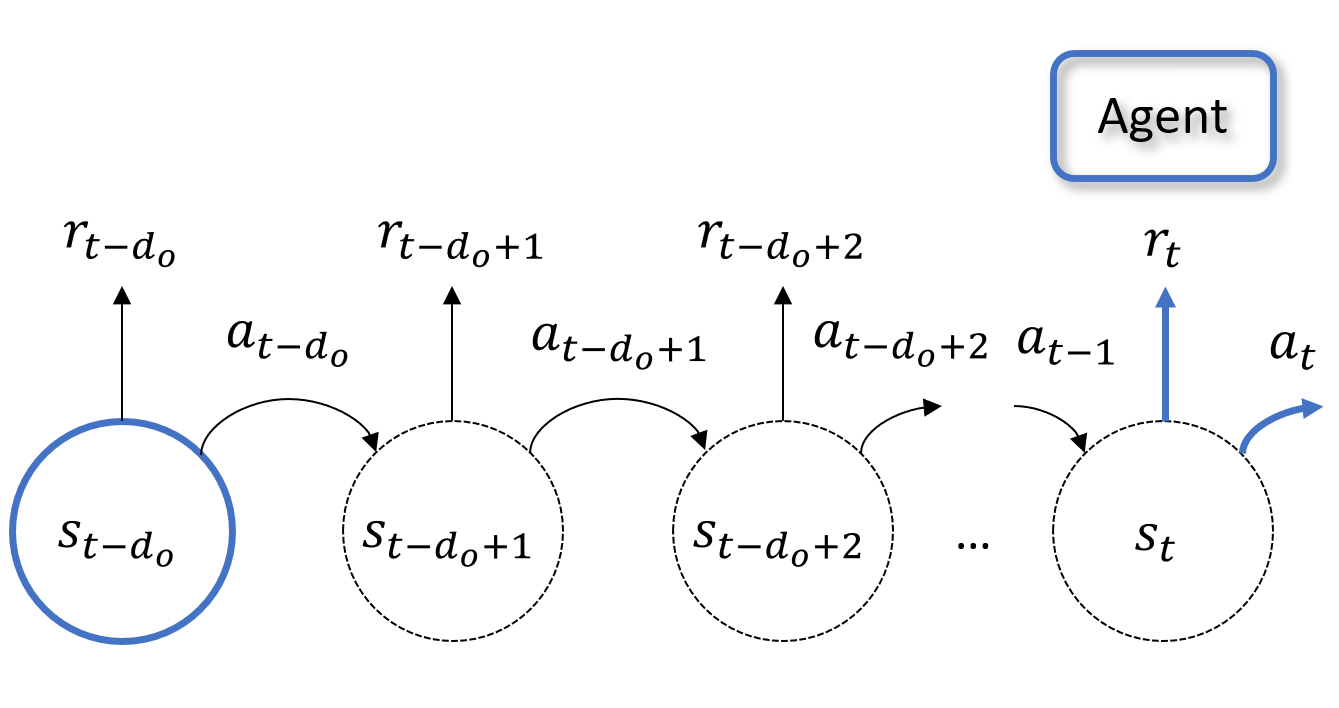
\includegraphics[width=11cm, keepaspectratio]{images/dmdp/o_delay.png}
                \caption{Observation Delay ($d_o$) effects. Agent's position is represented by the state aligned with it, while its perception is highlighted in light blue. The observed current state is $s_{t-d_{o}}$, but the actual current state is $s_{t}$.}
                \label{fig:o_delay}
                
                \vspace{0.5cm}
                
                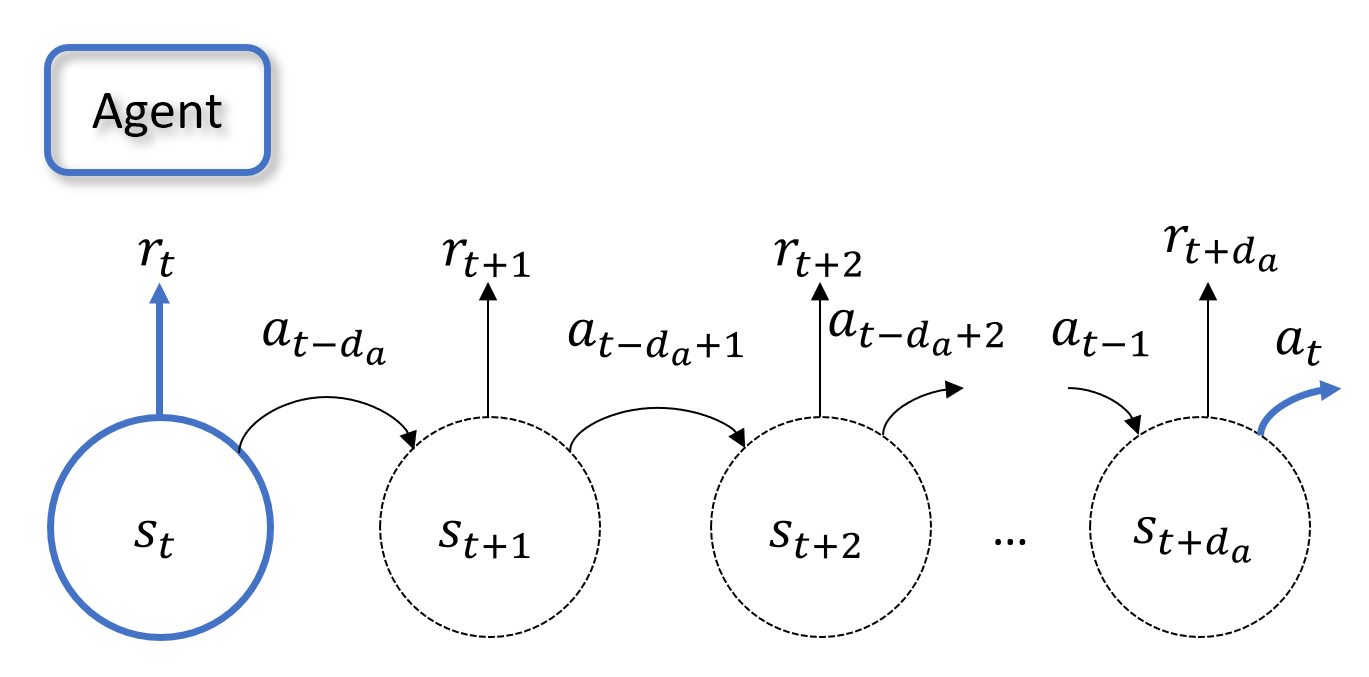
\includegraphics[width=11cm, keepaspectratio]{images/dmdp/a_delay.png}
                \caption{Execution Delay ($d_a$) effects. Agent's position is represented by the state aligned with it, while its perception is highlighted in light blue. The currently chosen action $a_t$ will actually take effect in $d_a$ steps, while the actual cause of the next transition is action $a_{t-d_{a}}$.}
                \label{fig:a_delay}
                
                \vspace{0.5cm}
                
                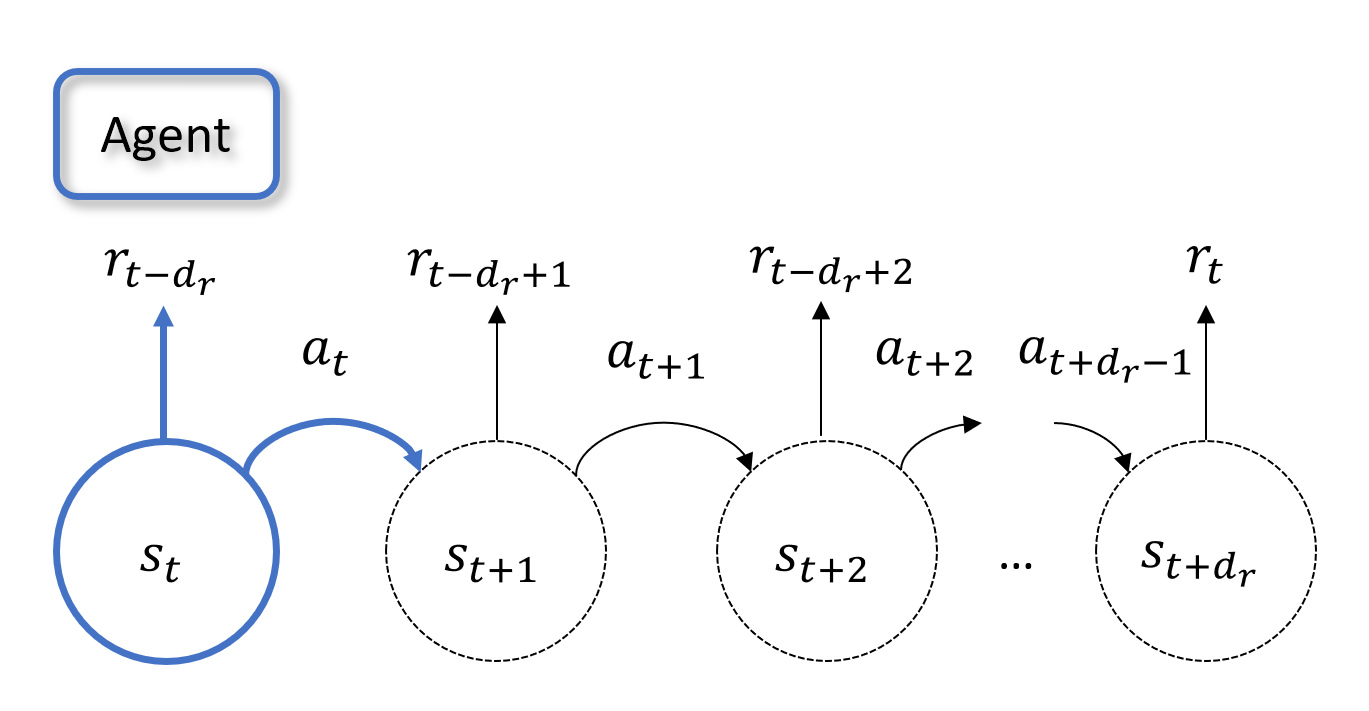
\includegraphics[width=11cm, keepaspectratio]{images/dmdp/r_delay.png}
                \caption{Reward Delay ($d_r$) effects. Agent's position is represented by the state aligned with it, while its perception is highlighted in light blue. The reward signal is collected $d_r$ time-step later w.r.t. the actual transition that generated it.}
                \label{fig:r_delay}
                
            \end{figure}
            
        \subsection{Delayed Markov Decision Process}
            Starting from the definitions of delays given the previous section, the MDP framework can be expanded in a straightforward manner, by including the delays:
            
            \begin{definition}[Observation Delayed MDP]
                \label{def:odmdp}
                An Observation Delayed MDP (or OD-MDP) is a 5-tuple:
                \[ \langle \mathbf{S}, \mathbf{A}, p, \mathbf{R}, d_o \rangle\]
                where $\mathbf{S}$ is the State Space, $\mathbf{A}$ is the Action Space, $p$ is the State-Transition Probability function, $\mathbf{R}$ is the Reward function and $d_o$ is the Observation Delay.
            \end{definition}
            \noindent
            In this definition, the term \textit{observation} is used as an alternative of the term state, although it may be more general in the sense that it also includes cases in which the state is not fully available to the Agent (i.e. Partially-Observable MDP).
            
            \begin{definition}[Execution Delayed MDP]
                \label{def:edmdp}
                An Execution Delayed MDP (or ED-MDP) is a 5-tuple:
                \[ \langle \mathbf{S}, \mathbf{A}, p, \mathbf{R}, d_a \rangle\]
                where $\mathbf{S}$ is the State Space, $\mathbf{A}$ is the Action Space, $p$ is the State-Transition Probability function, $\mathbf{R}$ is the Reward function and $d_a$ is the Execution Delay.
            \end{definition}
            
            \begin{definition}[Reward Delayed MDP]
                \label{def:rdmdp}
                A Reward Delayed MDP (or RD-MDP) is a 5-tuple:
                \[ \langle \mathbf{S}, \mathbf{A}, p, \mathbf{R}, d_r \rangle\]
                where $\mathbf{S}$ is the State Space, $\mathbf{A}$ is the Action Space, $p$ is the State-Transition Probability function, $\mathbf{R}$ is the Reward function and $d_a$ is the Reward Delay.
            \end{definition}
            \noindent
            Finally, the last three definitions can be combined in order to obtain a general definition that takes into account for every type of delay:
            
            \begin{definition}[Delayed MDP]
                \label{def:dmdp}
                A Delayed MDP (or DMDP) is a 7-tuple:
                \[ \langle \mathbf{S}, \mathbf{A}, p, \mathbf{R}, d_o, d_a, d_r \rangle\]
                where $\mathbf{S}$ is the State Space, $\mathbf{A}$ is the Action Space, $p$ is the State-Transition Probability function, $\mathbf{R}$ is the Reward function, $d_o$ is the Observation Delay, $d_a$ is the Execution Delay, $d_r$ is the Reward Delay.
            \end{definition}
            \noindent
            In general, the presence of delays can be represented by a mixture of the examples provided in Figures \ref{fig:o_delay}, \ref{fig:a_delay} and \ref{fig:r_delay}, showing a much more complex interaction between the Agent and the Environment than the MDP framework interaction. \newline
            The definition of Delayed MDP is the starting point in defining how the presence of delays can be modeled in order to fit within the already widely used MDP framework. However, it must be noted that, although it can cover a large variety of delays, it is not sufficient to describe an entire picture of the issue and how to properly solve it.
            
            \subsubsection{Time-Discretization Assumption}
                As \pcite{delay:memoryless} observe, there is no guarantee that the amount of time delay is an integer multiple of the sampling time that regulates the time discretization for the Agent. As such, delayed information and actuation may not be aligned with the ticks of time that the Agent is following. In fact, delays definitions (Definition \ref{def:obsdelay}, \ref{def:execdelay} and \ref{def:rewdelay}) measure the amount of delay in terms of an integer number of time-steps and they implicitly assume their alignment with the Agent discrete time. This assumption holds throughout this research and it allows for a stronger focus on other complications.
        
        \subsection{DMDP and Partially Observable MDP}
            \subsubsection{Markov Property in DMDP}
                \label{subs:markovmdp}
                As presented in Section \ref{subs:markov}, Markov Property (Definition \ref{def:markov}) represents the foundation upon which the entire MDP framework is based, along with all the collateral definitions. However, 
                Definitions \ref{def:odmdp} (OD-MDP) and \ref{def:edmdp} (ED-MDP) undermine the Markov Property implicitly. In fact, both OD-MDP and ED-MDP assume that the decision process taken by the Agent throughout its trajectories is based on a partial amount of information. \newline
                In an OD-MDP, the Agent is observing as current state $s_{t-d_{o}}$ which has been traversed a certain amount of time-step $d_o$ before and basing its decision-making process on it. This results in a violation of the Markov Property, because the past state $s_{t-d_{o}}$ does not constitute all necessary information regarding the previous interaction of the Agent with the Environment, but lacks of all the states traversed in the time-steps $t \in (t-d_{o}, t]$. Similarly, in an ED-MDP, the decision-maker is selecting actions which impact will take effect in a certain number of time-steps $d_a$ on an observed state $s_{t+d_{a}}$. Thus, the current state $s_t$ is not a sufficient to contain all necessary information in order to plan an action in $d_{a}$ time-steps, resulting again in a violation of the Markov Property. \newline
                Markov Property ensures that the Agent can plan its decisions using a sufficient amount of information, allowing a complete focus on the ability of the Agent of efficiently learning a well-performant policy. Introducing delays in the MDP formulation disrupts this assumption, introducing a new source of uncertainty and lack of knowledge, which in turn directly affects the performance of the Agent. This brings DMDPs close to Partially Observable MDP, which are also based on a decision-making process carried out upon incomplete information about the current state of the Agent and for this reason basic definitions from POMDP literature are here presented.
        
            \subsubsection{Partially Observable MDP}
                \label{subs:pomdp}
                Partially Observable MDPs (POMDPs) are a special class of MDPs in which the Agent does not perceive the complete state $s_t$, but rather an observation $o_t$ resulting from it. The said observation $o_t$ is related to the actual state $s_t$ by an \textit{Observation Function}:
                
                \begin{definition}[Observation Function]
                    \label{def:pomdp-obsf}
                    An Observation Function is a function that assigns the probability of being in a certain state $s_t$ knowing a certain observation $o_t$. It is denoted as:
                    \[ O : \mathbf{S} \times \mathbf{O} \rightarrow [0, 1] \]
                    \[ O(s_t | o_t) \]
                    where $\mathbf{S}$ is the State Space and $\mathbf{O}$ is the Observation Space (i.e. the Set of all the possible Observations $o$). 
                \end{definition}
                \noindent
                This entails that the decision process carried out by an Agent in a POMDP is not based on the certainty of observing a state, but rather on the probability of being in a certain state, given the observation perceived. This concept is formalized in the definition of Belief State:
                
                \begin{definition}[Belief State]
                    \label{def:pomdp-belief}
                    A Belief State $\mathbf{B}$ is a probability distribution over all the possible states in the State Space $\mathbf{S}$, given the history of the observations $o_t$.
                \end{definition}
                \noindent
                The presentation of this concepts is actually interesting since they constitute a relationship with the DMDP class. In both frameworks, the Agent is planning its decisions using incomplete knowledge of the Environment and, for example, the concept of Belief State could be applicable to the current unobserved state $s_t$ in OD-DMDP or to the future state $s_{t+d_{a}}$ in ED-MDP. \newline
                Thus, several topics of research in the field of POMDP represents an interesting inspiration in order to formulate new solutions for the presence of delay in DMDP. In fact, some of this topics have been used as starting point for several concepts in future sections of this research and a more in-depth analysis is presented in Section \ref{sota:pomdp}.
            
        \subsection{Deterministic and Stochastic Delays}
        \label{sub:dmdp_stochdelays}
            The definition of DMDP provided in Definition \ref{def:dmdp} explicitly assumes that the different kinds of delay can be formulated as a constant integer number that counts the number of time-steps of delay experienced by the Agent. This assumption represents another simplification of the nature of real environments. In fact, there exists no guarantee that the amount of delay, for each of the three presented kinds, will remain constant throughout all the trajectories the Agent can experience. \newline
            A number of events can occur that has an impact on the amount of delays perceived by the Agent, which may be due to the complex environment properties that involves different mechanisms' interaction. For example, the effectiveness of a medical procedure can be assessed by observing the patient conditions, which in turn are governed by complex biological and chemical processes that require an almost per use-case basis amount of time. Data transmission's delays are governed by the rules of queues and traffics on the networks, which are seldom constant throughout time. Thus, it is important to take notice that delays are not constant and a proper, more complex, formulation may be necessary depending on the Environment. 
            \\\\
            For this purpose, Definition \ref{def:dmdp} of a DMDP can be divided in two more specific definitions:
            
            \begin{definition}[Constant Delayed MDP]
                \label{def:cdmdp}
                A Constant Delayed MDP (or CDMDP) is a 7-tuple:
                \[ \langle \mathbf{S}, \mathbf{A}, p, \mathbf{R}, d_o, d_a, d_r \rangle\]
                where $\mathbf{S}$ is the State Space, $\mathbf{A}$ is the Action Space, $p$ is the State-Transition Probability function, $\mathbf{R}$ is the Reward function, $d_o$ is the Observation Delay, $d_a$ is the Execution Delay, $d_r$ is the Reward Delay. Furthermore, $d_o$, $d_a$ and $d_r$ are constant integer values.
            \end{definition}
            
            \begin{definition}{Stochastic Delayed MDP: }
                \label{def:sdmdp}
                A Stochastic Delayed MDP (or SDMDP) is a 7-tuple:
                \[ \langle \mathbf{S}, \mathbf{A}, p, \mathbf{R}, d_o(t), d_a(t), d_r(t) \rangle\]
                where $\mathbf{S}$ is the State Space, $\mathbf{A}$ is the Action Space, $p$ is the State-Transition Probability function, $\mathbf{R}$ is the Reward function, $d_o(t)$ is the Observation Delay, $d_a(t)$ is the Execution Delay, $d_r(t)$ is the Reward Delay. Furthermore, $d_o(t)$, $d_a(t)$ and $d_r(t)$ represents discrete-time stochastic processes.
            \end{definition}
            
            \subsubsection{Impact of Delay's Stochasticity}
            Introducing stochastic delays in the MDP framework can have several tricky consequences to be handled. For each kind of delay, sequentiality is not guaranteed anymore. Observations may be perceived in a different order based on the sampled delay at each time-step: supposing $d_o(0) = 3$ and $d_o(1) = 1$, state $s_0$ will be observed at time-step $t=3$, while state $s_1$ will be observed at time-step $t=2$. The same issue is present with Execution Delay $d_a(t)$, which affects the order on which actions take effect on the environment, and Reward Delay $d_r(t)$, which affects the order of reward collection. It may happen that the Agent observes different states at the same time-step, different actions take effect in the same time-step or different rewards are collected together. Furthermore, it may also happen to collect a reward from an unobserved state, implicitly revealing information about it. \\\\
            Careful assumptions can be made in order to circumvent some of this problematic and difficult behaviours. For example, \pcite{delay:dmdp} assumes that, at each time-step, the Agent can either receive a new observation or experience one more step of delay. They also assume that the probability of collecting a reward from an unobserved state is zero. In turn, this assumption entails that the delay experienced by the Agent can only grow indefinitely with time, leading to an undesired scenario in which the Agent needs to wait for it to be reduced. Other works such as \pcite{delay:mbs} and \pcite{delay:memoryless} assume constant delays, respectively explicitly and implicitly, as a reasonable middle-ground and, at last, another viable option is formulating the stochastic delays as a well-known stochastic process, such as Poisson distribution (\pcite{delay:mmqm}). \newline
            Throughout this research, both Deterministic and Stochastic Delays are studied and tested and, similarly, a number of assumptions and a formulation are used for Stochastic Delays. In particular, it has been assumed that the amount of Reward delay is always equal to the amount of Observation delay at each time-step, in order to avoid receiving information on an unobserved state through the reward signal.
        
        \subsection{Known and Anonymous Delays}
            In Reinforcement Learning, there is no guaranteed that the Environment properties are fully disclosed to the Agent or to the researcher that is implementing the Agent. This is valid for the dynamics of the system as much as for the delays of the system. In fact, information about the amount of constant delay or about the stochastic process that produces the delay may not be available at all or partly missing, as in the case in which several states are observed together or rewards is perceived as a sum of past rewards. The Agent is not able to understand from which time-step they are actually produced. In this case, the type of delay is said to be Anonymous and further steps must be taken in order to allow the Agent to learn the nature of the delay itself. Otherwise, if information about delays in the actual Environment is completely given or decided a priori for an Environment simulation, the delay is said to be Known. \newline
            For the purpose of this research, delays are known and simulated in the tested environments. This allows for a more focused study of the capability of the proposed method to act in presence of delay rather than of correctly assessing the amount and type of delay.
        